%% ------------------------------------------------------------------- %%
\chapter{Estado del Arte}
\label{cap:estadodelarte}
\lhead{\emph{Estado del Arte}} 

En este capítulo detallamos la metodología utilizada para realizar una Revisión Sistemática de la Literatura (RSL) referente a los métodos basados en Transformer y redes neuronales que utilicen mecanismos de atención para la detección de neoantígenos.

\section{Revisión Sistemática de la Literatura (RSL)}

Nuestro enfoque principal se centra en la priorización de neoantígenos (ver Figura 	\ref{fig:etapas}), ya que esta área ha sido objeto de una cantidad significativa de investigaciones que utilizan Transformers. Además, integramos análisis de pipelines y estudios de ensayos clínicos para obtener información sobre los hallazgos más recientes en cuanto a la aplicación de la detección de neoantígenos en vacunas personalizadas contra el cáncer. 

\begin{figure}[h]
	\centering	
	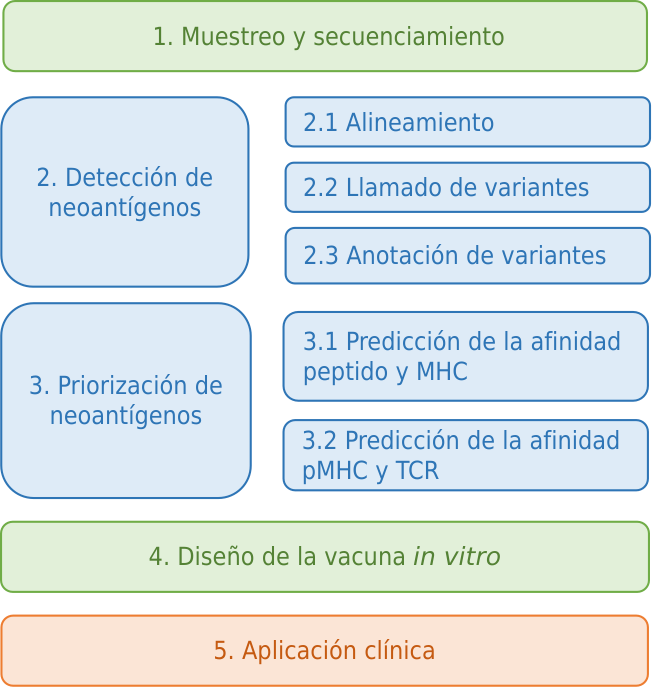
\includegraphics[width=0.5\textwidth]{img/pipeline/pipeline_spanish}	
	\caption{Una visión general de cada fase del proceso de generación de vacunas personalizadas basadas en neoantígenos.}
	\label{fig:etapas}
\end{figure}


Según las cadenas de búsqueda de la Tabla \ref{tab:search} y considerando solo trabajos publicados a partir de 2018, se analizaron los títulos de los artículos, obteniendo un total de 151 artículos. Luego, se seleccionó un subconjunto en función de los criterios de inclusión: artículos con una categoría ERA (A o B) o artículos de revistas en los cuartiles Q1/Q2. Al final de esta etapa, se obtuvieron 79 artículos.


\begin{table}
	\caption{Cadenas de búsqueda utilizadas en la RSL para cada fase de detección de neoantígenos.}
	\label{tab:search}
	\centering
	\setlength{\tabcolsep}{0.5em} % para el espaciado horizontal
	{\renewcommand{\arraystretch}{1.7}% para el espaciado vertical
		\begin{tabular}{p{3cm}p{10cm}}
			\textbf{Categoría} & \textbf{Cadena de búsqueda} \\ \hline
			Priorización de neoantígenos & (mhc OR hla) AND (peptide OR epitope OR antigen) AND (specificity OR immunogenicity OR binding OR affinity OR predict* OR detection OR presentation OR classification) AND (transformer* OR bert* OR attention OR 'transfer learning' OR method* OR predict*)'', ( tcr OR 't cell' OR t-cell) AND (mhc OR peptide OR epitope OR antigen) AND (specificity OR immunogenicity OR binding OR affinity OR predict* OR detection OR presentation OR classification) AND (transformer* OR bert* OR attention OR 'transfer learning' OR method* OR predict*) \\
			
	
			Pipelines & (pipeline OR toolkit) AND ( tcr OR 't cell' OR t-cell OR mhc OR hla OR peptide OR epitope OR antigen* OR neoantigen*) (pipeline OR tool* OR workflow OR application OR web* ) AND ( peptide OR epitope OR antigen* OR neoantigen* OR neoepito*) AND (immunotherapy OR detection OR identify* OR predict* OR presentation*)\\
			
			Ensayos clínicos &  (neoantigen OR neoepitope OR denditric cell) AND (vaccines OR immunology)
			
	\end{tabular}}
\end{table}




\section{Resultados de la RSL}

\subsection{Detección de neoantígenos}

La detección de neoantígenos se basa en la identificación inicial de candidatos, seguida de su posterior priorización. En esta sección, explicaremos el proceso de detección de candidatos a neoantígenos (etapa 2 en la Figura \ref{fig:etapas}).

Durante esta etapa, se utilizan datos de secuenciación de ADN (DNA-seq) y de ARN (RNA-seq) para identificar candidatos a neoantígenos. Sin embargo, en este campo, se han adoptado ampliamente varias herramientas bien establecidas, y los Transformers no se utilizan regularmente. En primer lugar, se encarga de tomar datos de DNA-seq, RNA-seq y \textit{Mass Spectrometry} (MS) como entrada. Luego, procede a alinear estas secuencias utilizando herramientas como BWA-MEM y Bowtie2. Además, STAR podría ser utilizado porque alinea muestras de tumores de manera más efectiva \citep{rubinsteyn2018computational}. La salida de esta etapa consiste en archivos de alineación BAM. Para la llamada de variantes, se podrían emplear MuTect y Strelka. Posteriormente, la información de ambos métodos se podría combinar, siguiendo el enfoque utilizado por \cite{zhou2021prioritizing} y \cite{rubinsteyn2018computational}. La salida consiste en archivos VCF. A continuación, está la etapa de anotación de variantes, donde se utilizan archivos con formato VCF para derivar péptidos generados a partir de estas variaciones o mutaciones; Isovar y ANNOVAR podrían ser utilizados en esta tarea. Finalmente, para determinar el tipo de HLA del paciente, la herramienta OptiType es una opción. Al final, tenemos varios candidatos a neoantígenos y los tipos de HLA del paciente.

\subsection{Priorización de neoantígenos}

La priorización de neoantígenos es la tercera etapa en el desarrollo de vacunas contra el cáncer (Figura \ref{fig:etapas}). En esta etapa, se toman los candidatos a neoantígenos y se predice su afinidad con el MHC, un problema conocido como predicción del enlace pMHC. Luego, este complejo pMHC se utiliza para predecir la interacción con el TCR. Ambos problemas toman dos secuencias de proteínas como entrada, y el objetivo es predecir su afinidad (regresión) o unión (clasificación). 


\subsubsection{Bases de datos}

Para priorizar neoantígenos, los investigadores a menudo recopilan muestras de diversas fuentes, generalmente extrayendo datos de estudios previos y recursos similares. Sin embargo, existen conjuntos de datos públicos disponibles, como se enumeran en la Tabla \ref{tab:bd}, que se centran específicamente en la interacción entre péptidos y MHC (péptido-MHC)  \citep{wu2018tsnadb, zhou2019neopeptide, tan2020dbpepneo, lu2022dbpepneo2}, así como en la interacción entre pMHC y TCR \citep{shugay2018vdjdb, bagaev2020vdjdb}. Es importante destacar que un estudio reciente proporciona estructuras tridimensionales de péptidos y HLA, lo que introduce una nueva perspectiva de investigación. Finalmente, la \textit{Immune Epitope Database} (IEDB) \citep{vita2019immune} se destaca como un recurso ejemplar en este campo.

\begin{table}[h]
	\caption{Bases de datos públicas de unión pMHC e interacción pMHC-TCR}
	\label{tab:bd}
	\setlength{\tabcolsep}{0.5em} % para el espaciado horizontal
	{\renewcommand{\arraystretch}{1.2}% para el espaciado vertical
		
		\begin{tabular}{lp{1cm}p{3.5cm}p{6cm}}
			\textbf{Nombre} & \textbf{Año} & \textbf{Ref.} & \textbf{Descripción} \\ \hline
			VDJdb           & 2018 & \cite{shugay2018vdjdb, bagaev2020vdjdb} & Base de datos de unión del TCR al pMHC, contiene 5491 muestras. \\
			IEDB            & 2018 & \cite{vita2019immune} & Es la base de datos más grande que contiene información de \textit{epitopes} de células T de humanos y otros organismos. \\
			TSNAdb          & 2018 & \cite{wu2018tsnadb} & Involucra 7748 muestras de mutaciones y HLA de 16 tipos de cáncer. \\
			NeoPeptide      & 2019 & \cite{zhou2019neopeptide} & Incorpora muestras de neoantígenos resultantes de mutaciones somáticas y elementos relacionados. También contiene 1818137 \textit{epitopes} de más de 36000 neoantígenos. \\
			
			pHLA3D          & 2019 & \cite{e2019phla3d} & Presenta 106 estructuras 3D de las cadenas $\alpha$, $\beta 2M$ y péptidos de las moléculas HLA-I. \\
			dbPepNeo        & 2020 & \cite{tan2020dbpepneo} & Contiene muestras validadas de la unión del pMHC a partir de MS. Incluye 407794 muestras de baja calidad, 247 de calidad media y 295 de alta calidad. \\
			dbPepNeo2.0     & 2022 & \cite{lu2022dbpepneo2} & Recopila una lista de neoantígenos y moléculas HLA. Presenta 801 HLAs de alta calidad y 842,289 de baja calidad. Además, 55 neoantígenos de clase II y 630 neoantígenos con unión al TCR. \\
			IntroSpect      & 2022 & \cite{zhang2022introspect} & Es una herramienta para construir bases de datos sobre la unión pMHC. Utiliza datos de MS. \\
			IPD-IMGT    & 2022 & \cite{robinson2020ipd} & Tiene 25000 moléculas MHC y 45 \textit{alleles}. \\
		\end{tabular}
	}
\end{table}

\subsubsection{Predicción de la unión pMHC}

Los enfoques para predecir la unión pMHC se pueden clasificar ampliamente en dos categorías: métodos \textit{allele-specific} y métodos \textit{pan-specific}. Los métodos \textit{allele-specific} implican entrenar un modelo distinto para cada \textit{allele} específico, mientras que los métodos \textit{pan-specific} implican el entrenamiento de un modelo universal aplicable a una variedad de \textit{alleles}. Luego, en la Tabla \ref{tab:transformes}, presentamos una comparación de modelos Transformer y métodos de aprendizaje profundo que utilizan mecanismos de atención.

Dado que trabajamos con entradas de proteínas, cada aminoácido se representa utilizando una fila de la matriz BLOSUM. Algunos estudios han utilizado BLOSUM62 \citep{jin2021deep, ye2021mathla, zhao2019peptide, o2018mhcflurry} y BLOSUM50 \citep{yang2021deepnetbim, hu2019acme}. Además, ciertos autores han utilizado una combinación de codificación one-hot y codificación BLOSUM \citep{liu2021deepseqpanii, jokinen2021predicting, zeng2019quantification, zeng2019deepligand}. Alternativamente, se han empleado métodos como el codificador universal de Google \citep{kubick2021predicting}, AAindex \citep{kawashima2000aaindex, li2021deepimmuno} (una base de datos de índices numéricos que representan propiedades fisicoquímicas y bioquímicas de los aminoácidos), coordenadas tridimensionales de aminoácidos \citep{shi2020deepantigen}, y la consideración de las propiedades fisicoquímicas de aminoácidos individuales \citep{moris2021current, montemurro2021nettcr, luu2021predicting}. Más recientemente, algunos estudios han incorporado ligandos eluídos de la membrana celular, extraídos mediante datos MS \citep{zhouprioritizing, reynisson2020netmhcpan, reynisson2020improved, o2020mhcflurry, alvarez2019nnalign_ma}.

Actualmente, NetMHCPan4.1 \citep{reynisson2020netmhcpan} es un método de referencia, este es una red neuronal artificial profunda  que consiste en 40 redes neuronales artificiales ensambladas; cabe destacar que maneja eficazmente conjuntos de datos de MS, al igual que el MHCflurry2.0 \citep{o2020mhcflurry}.

\begin{table}[ht]
	\caption{Transformers y métodos de aprendizaje profundo con mecanismos de atención utilizados para la predicción de la unión pMHC.}
	\label{tab:transformes}
	\setlength{\tabcolsep}{0.5em} % para el espaciado horizontal
	{\renewcommand{\arraystretch}{1.1}% para el espaciado vertical
		
		\begin{scriptsize}
			
		
		\begin{tabular}{p{2.5cm}p{2.5cm}p{2cm}p{5.5cm}}
			\multicolumn{1}{l}{\textbf{Ref.}}                                   & \textbf{Nombre}             & \textbf{Entrada}            & \textbf{Modelo}     \\  \hline
			
			\cite{hashemi2023improved}&	ESM-GAT  &	One-hot & BERT con transferencia de aprendizaje de ESM1b y ESM2 \textit{fine-tuned} con una \textit{Graph Attention Network} (GAT) al final. Superó a NetMHCpan4.1.	\\
			
			
			\cite{kalemati2023capsnet}&	CapsNet-MHC&	BLOSUM62 & \textit{Capsule Neural Network}, superó a las herramientas de vanguardia para péptidos pequeños de 8 a 11 mer.	\\
			
			\cite{ye2023stmhcpan}&	STMHCpan  &	One-hot & Un modelo Star-Transformer, útil para péptidos de cualquier longitud y ampliable para predecir respuestas de células T.	\\
			
			\cite{jing2023dapnet}&	DapNet-HLA&	\textit{Fused word embedding} & Combina las ventajas de CNN, SENet (para agrupación) y LSTM con atención.	\\
			
			\cite{zhang2022hlab}&	HLAB&	One-hot & BERT del modelo pre-entrenado ProtBert seguido de una BiLSTM.	\\
			
			\cite{wang2022mhcroberta}          & MHC RoBERTa            & One-hot & RoBERTa pre-entrenado seguido de 12 \textit{multi-head self-attention} y capas totalmente conectadas, superó a NetMHCPan3.0.                                                                                          \\
			\cite{chu2022transformer}          & TransPHLA             & One-hot         & Utiliza un mecanismo de self-attention basado en cuatro bloques, superó ligeramente a NetMHCpan4.1 y es más rápido en hacer predicciones.\\
			
			\cite{chen2021jointly}  & CapTransformer            & One-hot   &  Transformer con \textit{cross self-attention} para capturar información local y global.  \\
			
			\cite{gasser2021interpreting}  & ImmunoBERT            & One-hot                     & BERT de TAPE pre-entrenado seguido de una capa lineal. Los autores afirman que los terminales N y C son altamente relevantes después de un análisis con SHAP y LIME.   \\
			
			\cite{cheng2021bertmhc}             & BERTMHC              & One-hot                    & BERT de TAPE pre-entrenado seguido de una capa lineal. Superó a NetMHCIIpan3.2 y PUFFIN.   \\
			
			% CNN y RNN con atención
			\cite{ye2021mathla}         & MATHLA             & BLOSUM                      & 
			Integra BiLSTM con \textit{multi-head self-attention}. Obtuvo una puntuación AUC de 0.964, en comparación con 0.945, 0.925 y 0.905 para NetMHCpan 4.0, MHCflurry y ACME respectivamente  \\
			
			\cite{liu2021deepseqpanii}                    & DeepSeqPanII                            & BLOSUM62 y one-hot& Tiene dos capas LSTM, un bloque de atención y tres capas totalmente conectadas. Obtuvo mejores resultados que NetMHCIIpan 3.2 en 26 de 54 alelos.       \\
			
			\cite{yang2021deepnetbim}  & DeepNetBim               & BLOSUM50            & Utiliza CNN separadas para la predicción de la unión pMHC y \textit{immunogenetic} con un módulo de atención. Obtuvo 0.015 MAE para la unión y 94.7 de precisión para la inmunogenicidad.      \\
			
			\cite{jin2021deep}         & DeepAttention Pan        & BLOSUM62            & CNN con un mecanismo de atención. Es \textit{allele-specific} y obtuvo resultados ligeramente mejores que ACME a nivel de \textit{alleles}.     \\
			
			\cite{chen2021ranking}  & SpConvM            &  One-hot, BLOSUM y Deep                     &  Capa 1D de CNN, una capa de atención y una capa totalmente conectada. Además, emplearon \textit{global kernels} para mejorar sus resultados, junto con una combinación de onehot, BLOSUM y Deep.  \\
			
			\cite{venkatesh2020mhcattnnet}         & MHCAttNet        & One-hot            & CNN seguido de una capa de atención para generar un mapa de calor sobre los aminoácidos.     \\
			
			\cite{hu2019acme}          & ACME                     & BLOSUM50     & CNN con atención, extrae patrones interpretables sobre la unión pMHC. Además, obtuvo un SRCC de 0.569, un AUC de 0.9 para HLA-A y 0.88 para HLA-B.  \\    
			
			
			\cite{wu2019deephlapan}                      & DeepHLApan                              & One-hot             & Modelo \textit{allele-specific} con tres capas de GRU Bidireccional (BiGRU) con una capa de atención. Obtuvo una precisión $> 0.9$ en 43 \textit{alleles} HLA.                                               
		\end{tabular}
	\end{scriptsize}
	}
\end{table}

%CNN
Existen modelos de \textit{Convolutional Neural Networks} (CNN) que incorporan un mecanismo de atención, como ACME \citep{hu2019acme}. ACME utiliza una CNN con un módulo de atención que asigna pesos a posiciones de residuos individuales, con el objetivo de asignar mayores pesos a los residuos de mayor importancia en las interacciones pMHC. ACME logró un Coeficiente de Correlación de Rango de Spearman (SRCC) de 0.569, lo cual es superior a NetMHCpan 4.0. A continuación, tenemos MHCAttNet \citep{venkatesh2020mhcattnnet}, que utiliza una CNN seguida de una capa de atención. La capa de atención se utiliza para generar un mapa de calor sobre los aminoácidos, indicando las subsecuencias importantes presentes en la secuencia de aminoácidos. Otro modelo basado en CNN es DeepAttentionPan \citep{jin2021deep}, que utiliza una CNN profunda para codificar péptidos y MHC en vectores de dimensiones $40\times 10 \times 11$ antes de emplear un módulo de atención para calcular pesos posicionales. También contamos con DeepNetBim \citep{yang2021deepnetbim}, que incorpora un módulo de atención similar a ACME y DeepAttentionPan. Sin embargo, utiliza dos CNN separadas para predecir la unión pMHC y la inmunogenicidad, que luego se combinan en las capas finales. Además, en su estudio sobre SpConvM \citep{chen2021ranking}, los autores demostraron que la incorporación de núcleos globales en CNN con atención produjo un mejor rendimiento. Además, sus experimentos incluyeron una comparación de diferentes métodos de codificación de aminoácidos, incluyendo onehot, BLOSUM y Deep. Según sus hallazgos, la combinación de onehot, BLOSUM y Deep juntos dio como resultado mejores resultados. Recientemente, ha surgido el uso de \textit{Capsule Neural Network} (CapsNet) para modelar relaciones jerárquicas. CapsNet-MHC \citep{kalemati2023capsnet} se propone para predecir la unión pMHC-I, y superó a otras herramientas como HLAB, ACME, Anthem y NetMHCpan4.1 para péptidos pequeños de 8 a 11 mers.

% RNN
Además, se han introducido varias \textit{Recurrent Neural Networks} (RNN), como DeepHLApan \citep{wu2019deephlapan}, que es un modelo \textit{allele-specific} que considera datos de unión pMHC e inmunogenicidad. El modelo presenta tres capas de \textit{Bidirectional Gated Recurrent Unit} (BiGRU) y una capa de atención, produciendo finalmente las predicciones de unión e inmunogenicidad. Además, este enfoque incorporó epitopos de células T CD8+ y datos de MS; logró una precisión que supera 0.9 para 43 alelos HLA. Además, el modelo \textit{allele-specific} DeepSeqPanII \citep{liu2021deepseqpanii} utilizó una combinación de codificación BLOSUM62 y one-hot, con un enfoque específico en MHC-II. El modelo incluyó dos capas de \textit{Long Short-Term Memory} (LSTM) con 100 unidades y un bloque de atención para extraer información ponderada. El bloque de atención consistía en cuatro capas de convolución 1-D, y se emplearon tres capas completamente conectadas para predecir la afinidad. DeepSeqPanII superó a NetMHCIIpan 3.2 para 26 de los 54 \textit{alleles}. Otra RNN es MATHLA \citep{ye2021mathla}, que utilizó una BiLSTM para aprender las dependencias entre los residuos de aminoácidos y aplicó \textit{multi-head self-attention} para obtener información posicional para la salida de BiLSTM. La salida se procesó aún más a través de capas convolucionales 2-D. MATHLA logró un puntaje de AUC de 0.964, superando el rendimiento de NetMHCpan 4.0, MHCflurry y ACME, que obtuvieron puntajes de 0.945, 0.925 y 0.905, respectivamente. Recientemente, el modelo \textit{allele-specific} DapNet-HLA \citep{jing2023dapnet} introdujo un conjunto de datos adicional de Swiss-Prot para muestras negativas. El método utilizó un método de \textit{embedding} para cada token y su posición absoluta, que se comparó con varias técnicas de codificación, incluyendo la \textit{Desviación de Dipeptide Deviation from Expected mean} (DDE), \textit{Amino Acid Composition} (AAC), \textit{Dipeptide Composition} (DPC), y \textit{Encoding based on Grouped Weight} (EGBW). Recientemente, DapNet-HLA combinó las ventajas de CNN, SENet (para agrupamiento) y LSTM, logrando buenos resultados, aunque no se comparó directamente con métodos de vanguardia.


%BERT
BERTMHC \citep{cheng2021bertmhc} fue uno de los trabajos pioneros en incorporar la arquitectura BERT. Este predictor pan-específico de unión/presentación de pMHC-II utilizó el aprendizaje por transferencia de \textit{Tasks Assessing Protein Embeddings} (TAPE) \citep{rao2019evaluating}, un modelo entrenado con datos de la base de datos Pfam que comprende treinta y un millones de proteínas. Los autores integraron TAPE seguido de una capa \textit{Fully Connected} (FC). En experimentos, BERTMHC superó a NetMHCIIpan3.2 y PUFFIN, logrando un AUC de 0.8822 en comparación con 0.8774. Del mismo modo, ImmunoBERT \citep{gasser2021interpreting} aprovechó el aprendizaje por transferencia de TAPE, centrándose en la predicción de pMHC-I. El modelo tambien utilizo capas FC después del modelo TAPE. El análisis de los autores concluyó que los aminoácidos en proximidad a los extremos N/C del péptido son de alta relevancia, según análisis de LIME y SHAP. Además, CapTransformer \citep{chen2021jointly} introdujo un innovador mecanismo de \textit{cross self-attention} que alinea y agrega eficazmente las características de los residuos de pMHC de manera conjunta. Al utilizar tanto la \textit{self-attention} como \textit{cross self-attention}, facilita el aprendizaje de representaciones de características para los residuos individuales y la información global de unión pMHC, lo que resulta en un rendimiento superior en comparación con NetMHCpan4.0.



Otros métodos que utilizaron el aprendizaje por transferencia incluyen MHCRoBERTa \citep{wang2022mhcroberta} y HLAB \citep{zhang2022hlab}. El primero empleó cinco \textit{encoders} con doce \textit{multi-head self-attention}. Inicialmente, el enfoque utilizó un entrenamiento auto-supervisado con datos de las bases de datos UniProtKB y Swiss-Prot. El método también aplicó la tokenización de \textit{subtokens} y superó a NetMHCpan4.0 y MHCflurry2.0, logrando un coeficiente de correlación de Spearman Rank (SRCC) de 0.543. HLAB aprovechó el aprendizaje por transferencia de ProtBert-BFD \citep{elnaggar2021prottrans}, que fue entrenado con datos del conjunto de datos BFD que contiene 2,122 millones de proteínas. HLAB empleó un modelo BiLSTM al final de ProtBert-BFD y logró un rendimiento superior a  NetMHCpan4.1. Además, una investigación adicional examinó la aplicación del aprendizaje por transferencia y la aplicación de \textit{padding} \citep{arceda2023neoantigen}. Finalmente, TransPHLA \citep{chu2022transformer}  aplica la \textit{self-attention} a los péptidos, TransPHLA  supero a  NetMHCpan4.1, y ofrece la ventaja de ser efectivo para péptidos y \textit{alleles} de MHC de diferentes tamaños.

Una propuesta interesante implica el uso del modelo \textit{Star-Transformer}, SMHCpan \citep{ye2023stmhcpan}, un modelo liviano en el que la estructura de FC se reemplaza por una topología en forma de estrella. Además, las \textit{Graph Neural Networks} (GNN) se han utilizado en varios problemas de \textit{Protein-Protein Interaction} (PPI) debido a que gestionan las relaciones entre proteínas. En este contexto, surgió una propuesta novedosa, ESM-GAT \citep{hashemi2023improved}, que utilizó arquitecturas BERT y aprendizaje por transferencia de los modelos ESM1b y ESM2, luego apiló una \textit{Graph Attention Network} (GAT). Superó a NetMHCpan4.1; sin embargo, los autores no compararon la propuesta con otras herramientas del estado del arte.

\subsubsection{Predicción de la unión pMHC-TCR}


Los modelos, en general, tienen como entrada secuencias de TCR y pMHC. La representación de estos datos y la extracción de características son esenciales para obtener mejores resultados. Muchos modelos utilizan la matriz BLOSUM, mientras que algunos modelos emplean la codificación one-hot, y otros combinan BLOSUM y la codificación one-hot. Sin embargo, algunos optan por utilizar \textit{Granularity vectors} \citep{xu2022attntap}. 

\begin{table}[h]
	\caption{Métodos de Transformers y aprendizaje profundo con mecanismos de atención utilizados para la interacción pMHC con TCR.}
	\label{tab:TCR}
	\setlength{\tabcolsep}{0.5em} % para el espaciado horizontal
	{\renewcommand{\arraystretch}{1.1}% para el espaciado vertical
		
		\begin{scriptsize}
		\begin{tabular}{p{2.5cm}p{2.5cm}p{2cm}p{5.5cm}}
			\multicolumn{1}{l}{\textbf{Año}}                                   & \textbf{Nombre}          & \textbf{Entrada}              & \textbf{Modelo}     \\  \hline
			
			\cite{bravi2023transfer}	&	diffRBM	&	BLOSUM62	 &	Emplea una arquitectura RBM, aprendizaje por transferencia y \textit{Restricted Boltzmann Machines}.	\\%El modelo utiliza BLOSUM62
			
			\cite{10.1093/bioinformatics/btac820}	&	AVIB	&	BLOSUM50	&	Utiliza \textit{Attention of Experts} (AoE) (AoE) y \textit{multi-head self-attention} para predecir las interacciones entre TCRs y péptidos.	\\
			
			\cite{myronov2023bertrand}	&	BERTrand	&	BLOSUM62	&	Emplea un modelo BERT con más de 2.5 millones de parámetros, y utiliza una estrategia de pre-entrenamiento no supervisado para compensar la cantidad de parámetros.\\ %La entrada se representa mediante tokens, se convierte en una incrustación y se pasa a un cabezal de clasificación.
			
			\cite{zhang2023hybrid}	&	Hybrid gMLP 	&	BLOSUM50	&	Deep learning con mecanismos de atención para predecir la interacción de péptidos MHC y TCR, y puede manejar los problemas causados por las diferentes longitudes de los TCR.\\
			
		
			%2023\cite{wu2023tpbte}	&	TPBTE	&	BLOSUM62	&		\\%No está el artículo
			
			\cite{yang2023mix}	&	MIX-TPI	&	BLOSUM62	&	Emplea CNNs con \textit{self-attention} para construir un extractor basado en secuencias y características fisicoquímicas. Luego las fusiona con una capa de \textit{self-attention} para predecir las interacciones TCR-péptido.\\
			
			\cite{bradley2023structure}	&	TCRdock	&	BLOSUM62	&	Una versión especializada de AlphaFold para generar modelos de interacciones pMHC-TCR que se pueden utilizar para distinguir los \textit{epitopes} de los incorrectos. 	\\
			
			\cite{fang2022attention}	&	ATMTCR	&	BLOSUM50	&	ATMTCR se alimenta en dos capas completamente conectadas, un modelo \textit{Contrastive learning-based} y NetMHCpan para predecir la unión del TCR y el complejo pMHC.
			\\
			
			\cite{cai2022atm}	&	ATM-TCR	&	One-hot	\& BLOSUM &	Consta de dos \textit{encoders} y un \textit{decoder} lineal. % para determinar la afinidad de unión.
			Cada secuencia se alinea mediante IMGT. Calcula la similitud de los mapas de atención y los mapas de referencia para confirmar si hay una unión.\\
			
			\cite{xu2022attntap}	&	AttnTAP	& Vectores de Granularidad	&	Incluye una red BiLSTM, con mecanismos de atención y un perceptrón multicapa para extraer las características del TCR y el péptido y predecir la unión pMHC-TCR.\\
			
			%2022\cite{liu2021deepseqpanii}	&	DeepSeqPanII	&	One-hot \& BLOSUM62	&   
			%La arquitectura consta de codificadores de secuencias (RNN-LSTM con mecanismo de atención), un extractor de contexto de unión y un predictor de afinidad. Cada codificador tiene un módulo de atención.\\
			
			\cite{9994875}	&	pMTattn	&	Incrustación	&	Emplea cross \textit{self-attention} para aprender información de interacción entre pMHCs y TCRs. 
			\\
			
			\cite{xu2021dlptcr}	&	DLpTCR	&	One-hot	&    DLpTCR consiste una red totalmente conectada, LeNet-5 y ResNet-20 para predecir la unión péptido-CDR3$\alpha$($\beta$). También implementa un mecanismo de atención en ResNet-20.% para mejorar la calidad de las salidas generadas.
			\\
			
		
			
			%2021\cite{chen2021jointly}	&	capTransformer	&		&	Uses self and cross attentions for local embedding. Introduces a new cross attention pooling (caPool) with an outer concatenation operation to construct the Vcat matrix.% carrying residue-residue pair information. %It is already included
			%\\
			
			
			
			
			
		\end{tabular}
		\end{scriptsize}
}
\end{table}

%CNN
Las CNN con mecanismos de atención se emplean porque capturan y procesan eficazmente los datos. MIX-TPI \citep{yang2023mix}, un marco computacional multimodal, utiliza CNN con \textit{self-attention}. Tambien, se utilizan para construir \textit{sequence-based extractors} (SE) y \textit{physicochemical-based extractors} (PE), que se encargan de aprender características refinadas de secuencias y características fisicoquímicas, respectivamente. Finalmente,  \textit{self-attention} se emplea para fusionar estas representaciones y predecir la unión pMHC-TCR.

Por otro lado, las RNN realizan tareas que involucran datos secuenciales de aminoácidos de TCR y pMHC, y existen varios estudios de RNN con mecanismos de atención, como DLpTCR \citep{xu2021dlptcr} y AttnTAP \citep{xu2022attntap}. DLpTCR es un conjunto de tres arquitecturas de aprendizaje profundo que incluyen \textit{Fully Connected Layers} (FCN), LeNet-5 y ResNet-20 para predecir la probabilidad de interacción péptido-TCR y utiliza un mecanismo de atención en ResNet-20 para mejorar la calidad de las salidas generadas. AttnTAP es un marco de aprendizaje profundo de doble entrada que incluye una BiLSTM y una perceptrón multicapa (MLP), y un mecanismo de atención para extraer características de TCR y péptidos por separado y realizar la predicción de la unión péptido-TCR. Algunos estudios utilizaron CNN, RNN y mecanismos de atención, como TcellMatch \citep{fischer2020predicting}. TcellMatch es un conjunto de modelos de aprendizaje profundo con múltiples arquitecturas y utiliza una tecnología llamada de \textit{single-cell}, que permite la secuenciación simultánea de las cadenas TCR $\alpha$ y $\beta$ y la determinación de la especificidad de las células T. Este estudio también realiza múltiples comparaciones y demuestra que los modelos que incluyen tanto la cadena $\alpha$ como la cadena $\beta$ tienen una ventaja predictiva sobre los modelos que solo incluyen la cadena $\beta$, aunque la diferencia es pequeña pero significativa.
%RNN

%transformers
En la actualidad, se han desarrollado una variedad de modelos basados en Transformers. ATM-TCR \citep{cai2022atm} introdujo el uso de mecanismos de atención como parte principal y presentó un modelo que utiliza una red de \textit{multi-head self-attention}. Este modelo consta de dos \textit{encoders} para secuencias de TCR y \textit{epitopes} y un \textit{decoder} lineal para determinar la unión. Utiliza una red de \textit{multi-head self-attention} para obtener representaciones contextuales de cada secuencia. Cada una de las secuencias de TCR y \textit{epitopes} se alinea a través de IMGT y se utiliza la distancia euclidiana para calcular si hay unión o no. Luego, AVIB \citep{10.1093/bioinformatics/btac820}, una generalización de múltiples secuencias del \textit{Variational Information Bottleneck}, introdujo un novedoso método llamado \textit{Attention of Experts} (AoE). AoE puede aprovechar los abundantes datos disponibles cuando falta la secuencia de la cadena CDR3$\alpha$ o CDR3$\beta$. Tambien surge BERTrand \citep{myronov2023bertrand}, la arquitectura, BERT, se pre-entreno y realizo \textit{fine-tuning} para la predicción de la unión péptido-TCR. Inicialmente, los péptidos y TCR se representan como secuencias de tokens, y cada péptido y TCR se concatenan en una secuencia unificada que conserva su información posicional y tipológica. Otro modelo es Hybrid gMLP \citep{zhang2023hybrid} que combinó el modelo gMLP con el mecanismo de atención, donde la información se obtuvo a través de gMLP, y luego se utilizaron \textit{multi-head self-attention} y \textit{local attention} para extraer la información de correlación del CDR3 pMHC-TCR. Este marco puede manejar los problemas causados por diferentes longitudes de TCR. Además, demostró que los modelos entrenados con datos emparejados de cadenas CDR3-$\alpha$ y CDR3-$\beta$ son mejores que aquellos entrenados solo con datos de CDR3-$\alpha$ o CDR3-$\beta$. Este modelo puede tener potencial, pero le falta una base de datos grande para introducir su modelo poderoso. Finalmente, TCRdock \citep{bradley2023structure} es una versión especializada del predictor de redes neuronales AlphaFold, que demuestra que el predictor AlphaFold se puede utilizar para distinguir con precisión los \textit{epitopes} de péptidos correctos de los incorrectos. 

Otros métodos que utilizaron el aprendizaje por transferencia incluyen diffRBM \citep{bravi2023transfer} y pMTattn \citep{9994875}. DiffRBM es un enfoque basado en secuencias que utiliza aprendizaje por transferencia y \textit{Restricted Boltzmann Machines} RBM. Las RBM se utilizan principalmente en la representación y generación de datos. Este enfoque depende de dos conjuntos de datos diferentes genéricamente denominados conjuntos de datos ``selected'' y ``background'' de gran tamaño. Ambos conjuntos se entrenan con el modelo de RBM. pMTattn fue uno de los primeros modelos en adoptar un mecanismo de \textit{cross-attention}, lo que permite centrarse en los sitios de unión importantes. 


\subsection{Pipelines}
\subsection{Ensayos clínicos}

